\section{Verification of BoSSS for Inviscid Flows}
\frame{\tableofcontents[currentsection]}
\begin{frame}
	\frametitle{Problem Specification}
	
			\begin{columns}[t]
				\column[]{4cm}
				\vspace{-0.5cm}
				\begin{itemize}
					\bluedot Supersonic inlet
					\reddot Adiabatic slip wall
				\end{itemize}
				\begin{itemize}
					\item Flow properties:
					\begin{itemize}
						\item Symmetrical flow
					 	\item Isentropic inviscid flow with $\tfrac{p}{\rho^\gamma}=\text{const}$ \newline \MVRightarrow \, Entropy $s = 0$				
					\end{itemize}
				\end{itemize}
				\column[]{8cm}
				\begin{figure}[htbp]
					\vspace{-1cm}
					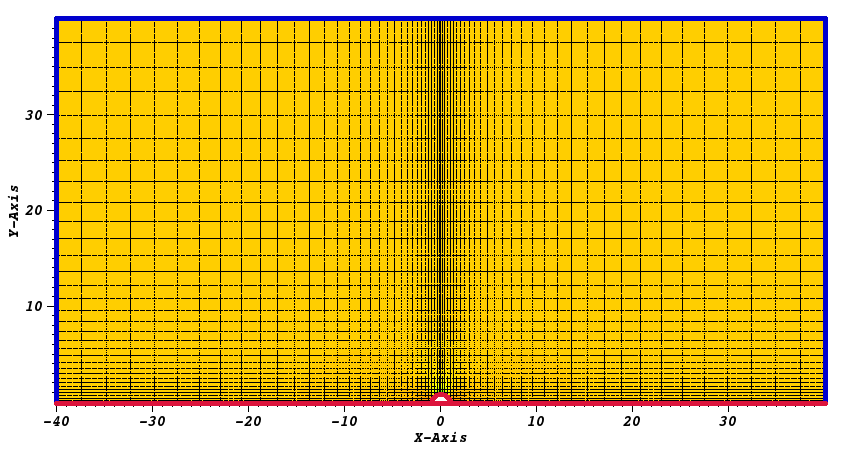
\includegraphics[width=\textwidth]{img/inviscid2.PNG}
					\vspace{-0.3cm}
					\caption{Mesh with 64 Cells per Direction}
				\end{figure} 
			\end{columns}
				\vspace{-0.8cm}
				\begin{itemize}
						\item Domain:
					\begin{itemize}
						\item $0 \leq y \leq 40$
						\item $-40 \leq x \leq 40$
						\item Cylinder with radius $r=1$ at $(0,0)$\newline \MVRightarrow \, Level set $\varphi  = x^2 + y^2 -1$ set as \color{myred} adiabatic slip wall\color{black}			
					\end{itemize}
				\end{itemize}

\end{frame}
	\subsection{Robustness}
	\begin{frame}
		\frametitle{Robustness Study -- Preparation}
		\begin{itemize}
			\item Variation of polynomial degree $ 1 \leq P \leq 3$
			\item Variation of position of the cylinder's centre point from $-0.075$ to $+0.075$ with step size $0.015$ \newline \MVRightArrow \, Level set $\varphi  = (x-\text{shift)}^2 + y^2 -1$
			\item Mesh as shown before (64 cells per direction)
			\item Constant agglomeration threshold $\alpha = 0.5$  \newline \MVRightArrow \, several different cell agglomerations occur			
		\end{itemize}
		\vspace{0.5cm}
		\begin{center}
			\large
			\textbf{Aim:} Proving the robustness of the solver
		\end{center}
	\end{frame}
	\begin{frame}
		\frametitle{Robustness Study -- Evaluation}
		\begin{columns}[t]
	\column[]{6cm}
		\vspace{-0.5cm}
	\begin{itemize}
		\item Constant error of entropy for degrees 1 and 2 \newline \MVRightarrow \, Only slight influence by cell agglomeration
		\item Large error differences for degree 3
		\begin{itemize}
			\item For some cases huge effort in getting calculations to work (early breakup)
			\item Discordant cases should be examined more closely
		\end{itemize}
	\end{itemize}
	\column[]{6cm}
			\begin{figure}[htp]	
				\vspace{-1cm}
				\centering
				\includestandalone[width=\textwidth]{shift}
			\end{figure}
		\end{columns}
	\begin{center}
		\large
		\MVRightarrow \, Sufficiently robust for lower degrees, higher degree calculations strongly influenced by cell agglomeration
	\end{center}
%		Ergebnisse, Plot, komischer punkt wird angeschaut
	\end{frame}
	\subsection{Convergence}
	\begin{frame}
		\frametitle{Comvergence Study -- Preparation}
		\begin{itemize}
			\item Variation of polynomial degree $ 0 \leq P \leq 4$
			\item Variation of mesh size: 32, 64 and 128 cells per direction
			\item Constant level set $\varphi  = x^2 + y^2 -1$
			\item Constant agglomeration threshold $\alpha = 0.3$
		\end{itemize}
		\vspace{0.5cm}
		\begin{center}
			\large
			\textbf{Aim:} Proving convergence rate of $\mathcal{O}(h^{P+1})$
		\end{center}
	\end{frame}
	\begin{frame}
		\frametitle{Convergence Study -- Evaluation}
		\begin{columns}[t]
			\column[]{4cm}
			\begin{itemize}
				\item Bad convergence rate for $P=0$
				\item Convergence of roughly $\mathcal{O}(h^{P+1})$ for $ 1 \leq P \leq 4$
			\end{itemize}
			\column[]{8cm}
		\begin{figure}[htp]
			\vspace{-1cm}
			\centering		
			\includestandalone[width=\textwidth]{convergence}
		\end{figure}
		\end{columns}
			\begin{center}
				\large
				Convergence rate for higher degrees as expected \newline \MVRightarrow \, Convergence verified
			\end{center}
	\end{frame}